\documentclass{article}

\usepackage{array}
\usepackage[rightcaption]{sidecap}
\usepackage{graphicx}
\usepackage{float}
\usepackage[utf8]{inputenc}
\usepackage[english]{babel}
\usepackage{cite}
\usepackage{listings}


\graphicspath{ {./images/} }

\begin{document}
\begin{center}
\thispagestyle{empty}
\parskip=14pt%
\vspace*{3\parskip}%
Meerkats File Synchronizer - Final Report

By

Made in GB

Boyang Zhang, Xi He, YiFeng Zheng,
 Yenan Huang, Frida Solheim \& Samah Alghamdi

For 7CCSMGPR GROUP PROJECT

Department of Informatics, King's College London

Term 2 2019
\end{center}
\newpage


\tableofcontents
\newpage

\section{Introduction}
We live in a dynamic and fast paced world where access to data is no longer limited to having access to a single device. Information is now available and accessible through one click and people are carrying small computers in their hands most of the time by having smart phone devices and are able to access their files from anywhere in the world. Additionally, enterprises use the cloud as a tool for collaboration to increase their workforce productivity and to meet their customers’ requirements of having mobile access to products and services.

Digital age and user mobility have made data availability crucial, not only for individuals, but for business alike. Demands for having timely access to data and to ensure data accuracy and redundancy have increased dramatically and the need for technical solutions to meet these requirements has risen accordingly. The solution to reduce the time and efforts that are needed to manage data among different devices and in different locations is by using file synchronization software. File synchronization software is used to ensure that files in two or more locations are updated via certain rules. Additionally, it is used for backup and for mobile access to files.


\hfill \break
In this project, we are embarked on a new journey where we develop a file synchronization software. We aim to provide a secure and seamless synchronization solution to enable data management processes, such as file creation, deletion, modification, distribution, redundancy and availability.

Our solution targets different kind of users and can be used in different sectors of the business world, such as health organizations, educational entities, financial companies and more. A company's employees for instance, who work at separate locations, can use it to access and distribute files. Individuals can utilize it to upload their holiday photos, for example, and to view them from their different devices.

We have chosen to name our software Meerkats, because the meerkats are one of the most collaborative animals in the world, and one of the main features for our software is collaboration.

\begin{figure}[h]
    \centering
    
\includegraphics[width=0.95\textwidth]{logo}
    \caption{Meerkats Logo}
    \label{fig:logo1}
\end{figure}

In this report, we provide information about the file synchronization software project. Detailing information about how we worked together as a team to develop our product, the strategies we used to ensure the delivery of reliable and efficient solution. We will also cover information about the features and the configuration of the software itself, in addition to our future plan.


\section{Review}
File synchronization softwares are popular and the most famous ones are Dropbox, GoogleDrive, One Drive and Box. We have reviewed these popular solutions. We found them all to provide the same basic features, as they allow users to access, share and synchronie data. Choosing the right synchronization software really depends on the user's needs and expectations, as each solution has its advantages and disadvantages. We have focused on the file synchronization feature in each solution to understand how it works.

\subsection{GoogleDrive}
\textbf{Storage and Cost:}
Signing up for GoogleDrive provide users with 15GB of storage space for free. It can be increased up to 1TB for 10 USD a month. Google Drive lets users automatically copy files onto their different devices.


\hfill \break %keep this break
\textbf{File Synchronization:}
The solution is compatible with Windows, Mac, Android and iOS. It implements a sync folder mechanism, adding a “Google Drive” folder to the user's file-system when they install the desktop client. Any folders or files the users choose to drop in the Google Drive folder gets sent off to the cloud, then onto other devices. The disadvantage of this process is that it requires the files be stored on both the users hard drive and in the cloud. This is not useful if the users want to free up their disk space. To address this concern, Google has introduced a new feature that allows users to select specific folders to help them free up hard drive space.

\subsection{Dropbox}
\textbf{Storage and Cost:}
Users who sign up to Dropbox gets 2GB of storage for free. This limited space is considered as a disadvantage of using Dropbox. If users want to get extra disk space, such as 100GB, they need to get a paid subscription plan for 10 USD a month.


\hfill \break
\textbf{File Synchronization:}
Dropbox can be installed on Windows, Mac, Linux, Android, iOS, Windows Phone, BlackBerry and Kindle Fire. As with GoogleDrive, Dropbox uses a sync folder with a new feature called block-level sync. This feature allows users to manage selective files stored in the sync folder from the “preferences” tool accessible via the DropBox taskbar icon (on PC). This is a very important functionality, as it helps users to save their disk space and to better utilize it to store important documents that they want to access and share from anywhere.


\subsection{Box}
\textbf{Cost and Storage}
Box for personal use offers free storage up to 10GB. Users can upgrade is they want  more flexibility and storage space (up to 100GB), which costs 10 USD per month.

\hfill \break
\textbf{File Synchronization}
Box applies the same file synchronization method invented by Dropbox. Adding files and folders to the Box Sync folder on a computer will automatically upload them tothe user's account on Box and mark them for Sync. Users can selectively sync folders to better manage their disk space. The solution can be run on Windows, Mac, Android, iOS, Windows Phone and BlackBerry.

\subsection{OneDrive}
\textbf{Cost and Storage}
OneDrive is a Microsoft product and it offers up to 5GB of free storage space. Users can pay 2 USD a month to increase the storage space to 50GB. The solution is a great productivity tool since it is integrated with many other Microsoft products, such as Office Online, Skype, Outlook and the Office 365 suite for desktop.

\hfill \break
\textbf{File Synchronization}
OneDrive can run on Windows, Mac, Android, iOS and Windows Phone. It follows the standard sync model developed by Dropbox. It includes a sync folder, which is like a normal folder with the only difference being that it's connected to the cloud. OneDrive offers a simple way to sync files. Users can move individual files to the OneDrive sync folder by right-clicking and selecting “move to OneDrive”. A drawback about OneDrive is that specific files can’t be synced to OneDrive. Instead, users have to go to the settings menu of the OneDrive desktop client and update the folders.

OneDrive is compatible with Google docs and with some other office tools. This provides convenience for users who have google accounts, as they can save their attachments directly into their googleDrive.
\newline
\hfill \break
We also looked at some resources such as Open Web Application Security Project (OWASP) to learn more about the risks associated with web applications, secure software development and cloud and file security.

\section{Requirements and design}
The requirements of this project have been supplied by the project's supervisor, Dr. Laurance, for which the team has precisely aligned the software design, project timeline and allocated resources to meet the expectations.

\subsection{Project Deliverables}
By completing this project, the following deliverables are achieved.
\begin{enumerate}
  \item \textbf{File Storage Server} This component is used to store files and deal with requests received from users.
  \item \textbf{Mobile Client} It is an Android solution. Users can use the app on the go and will enjoy features such as Sign Up, Log In, View Files, Upload Files, Rename Files, Delete Files, etc.
  \item \textbf{Desktop GUI Client} The desktop GUI client is based on the Windows OS and it includes the same features as the mobile client.
  \item \textbf{Meerkats File Synchronizer Report} This report provides detailed information about the project in terms of team members, project plan, deliverables, timeline, technologies used, challenges and much more. It acts as a central reference for users who are interested in the software.
  \item \textbf{Meerkats File Synchronizer Presentation} The team will put together slides to present the work done. The team will demonstrate the solution and its layout, features and will walk the audience through the function- alities supplied by the software.
\end{enumerate}


\subsection{Business Requirements}
POSSIBLY MERGE THIS WITH DELIVERABLES
ADD SOME SORT OF INTRO HERE
\begin{enumerate}
  \item Develop File Synchronization Software
  Description:  File synchronization software is used to store copies of files to another device or to the cloud. The files are typically available to be accessed via a Web-based portal. Some examples of file sync software include Box and Dropbox.
  \item Build a ‘hub and spoke‘ file synchronizer
  Description: File synchronizer will allow communication between a single central server (the ‘hub’) to which multiple other clients (the ‘spokes’) synchronize.
  \item Develop a web server and two clients (desktop, mobile)
  Description: A web server will be developed and it will exchange data with mobile client (Android) and desktop client (Windows).
\end{enumerate}


\subsection{Project plan}

\begin{figure}[h]
    \centering
    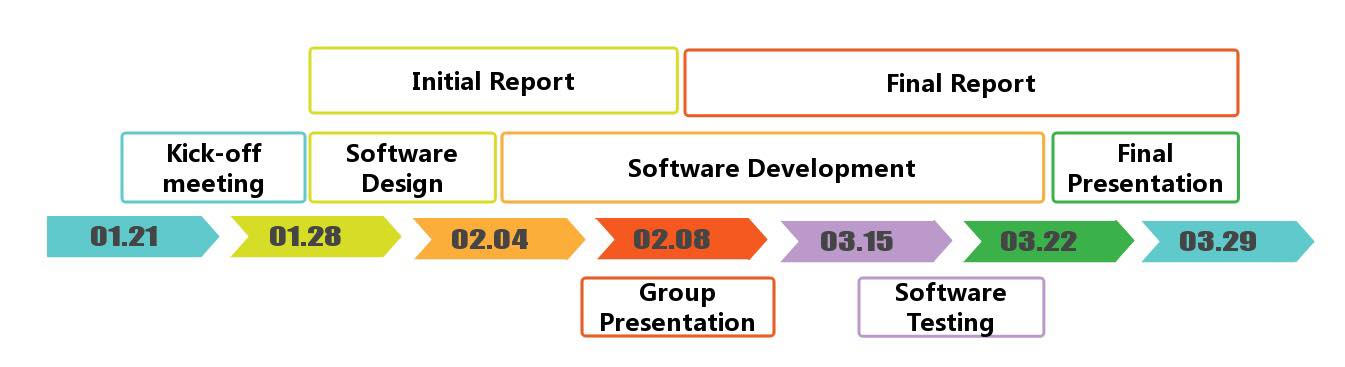
\includegraphics[width=1\textwidth]{timeline}
    \caption{Timeline}
    \label{fig:timeline1}
\end{figure}

TALK ABOUT TIMELINE.

\subsection{Implementation Timeframe}
Below table outlines the milestones along with brief description and expected timeframe.

\begin{center}
\begin{tabular}{ | m{3em} | m{2cm}| m{3cm} | m{1cm} | m{1cm} | m{2cm} |}
\hline
\textbf{\#} & \textbf{Milestones} & \textbf{Description} & \textbf{Start Date} & \textbf{End Date} & \textbf{Status}  \\
\hline
1 & Kick-off meeting & Background survey and initial plan & Jan 21, 2019 & Jan 27, 2019 & Completed \\
\hline
2 & Software Design  & Design the software layout & Jan 28, 2019 & Feb 3, 2019 & Completed \\
\hline
3 & Software Development & Work to deliver the file synchronization software & Feb 4, 2019 & March 21, 2019 & Completed \\
\hline
4 & Initial Report & To develop and submit the initial report & Jan 29, 2019 & Feb 7, 2019 & Completed \\
\hline
5 & Group Presentation & To demonstrate  the group initial software design and share the project plan & Feb 8, 2019 & Feb 8, 2019 & Completed \\
\hline
6 & Software Testing &  To test the software and ensure correct and secured implementation & March 15, 2019 & March 21, 2019 & Completed \\
\hline
7 & Final report & To submit the final report describing complete information about the software and the project lifecycle & Feb 8, 2019 & March 28, 2019 & Completed \\
\hline
8 & Final Presentation & To deliver the final presentation about the software & March 22, 2019 & March 29, 2019 & In progress \\
\hline
\end{tabular}
\end{center}

\subsection{Design Model}
The team has decided to follow the strategy of capitalizing on existing experiences and skills to save time and to deliver an efficient solution. Some of the team members had the opportunity to develop android applications and others had the chance to build windows applications. Therefore, it was wise to go with those platforms since the expertise already exists in the group. These systems are also reliable and widely used by users.

The following flow charts show the general design of the solution as well as detailed design for the Android and Windows clients.


\subsection{Mobile Application Interface Design Principles}
We understand that designing mobile applications is very different than designing desktop applications. Therefore we got into a mobile design "mindset" before starting the design of the mobile app.
We designed the mobile client interface with great intent to impress users within the few seconds after they start using it and to retain them in the long run. We tried our best to create an excellent User Experience (UX). For that, we have searched the Internet and learned about UX and how it contributes to the success of any new application. We also spent much time in searching and looking for a variety of design examples for inspirations. We have come up with intuitive and creative mobile interface design where we have followed collection of interface design principles that include but not limited to:

\begin{enumerate}
\item \textbf{Consistency of the design layout:} We made sure to design the sections of the application to be coherent, and we provided a consistent flow of the layout throughout the app.
\item \textbf{Unambiguous Interactive Elements:} Elements that are intended for interaction with users are clearly depicted. Key options such as Create, Delete and Rename are visible and easy to access by users when required by them without the need to search for hidden options in menus.
\item \textbf{Single Trial Learning Experience:}  Since we aim to create user friendly application, we designed the app and placed the options tin a way that allow users to anticipate the next step and the flow of the process in general without the need to remember the steps.
\item \textbf{Layered User Experience:} We understand that UX should be layered. Meaning that not all the features and options of the app are visible at once. We kept some buttons hidden as we wanted to keep the interest of users for longer time and as they go deeper into the app. However, we balanced between keeping the excitement of users and the simplicity of navigating the app.
\item \textbf{Navigation Models:} We know that there are many navigation models out there but we chose Drill down because it makes the most sense of our application.
\item \textbf{Orientation:} We have selected portrait and landscape to follow the user's hands movement.
\item \textbf{Launching:} When users launch the application, they will see an image that represent the logo of the software and the application name only. We aimed at not to confuse users at the beginning by adding buttons and text when they firs load the application. When users leave the app and comeback to it, they will resume operation right where they left the application.
\item \textbf{First impressions:} We believe on the say “ first launch make or break situation” therefore, we though of the following things:
\end{enumerate}
\begin{itemize}
\item \textbf{Icons:} We have kept text to minimum, and selected polished and eye attraction icons to attract users attention and create excellent and lasting first impression.
\item \textbf{First launch:} We ensured that users are not lost when they first launch the application and can easily deal with it without the need to seek assistance.
\end{itemize}

\begin{figure}[h]
    \centering
    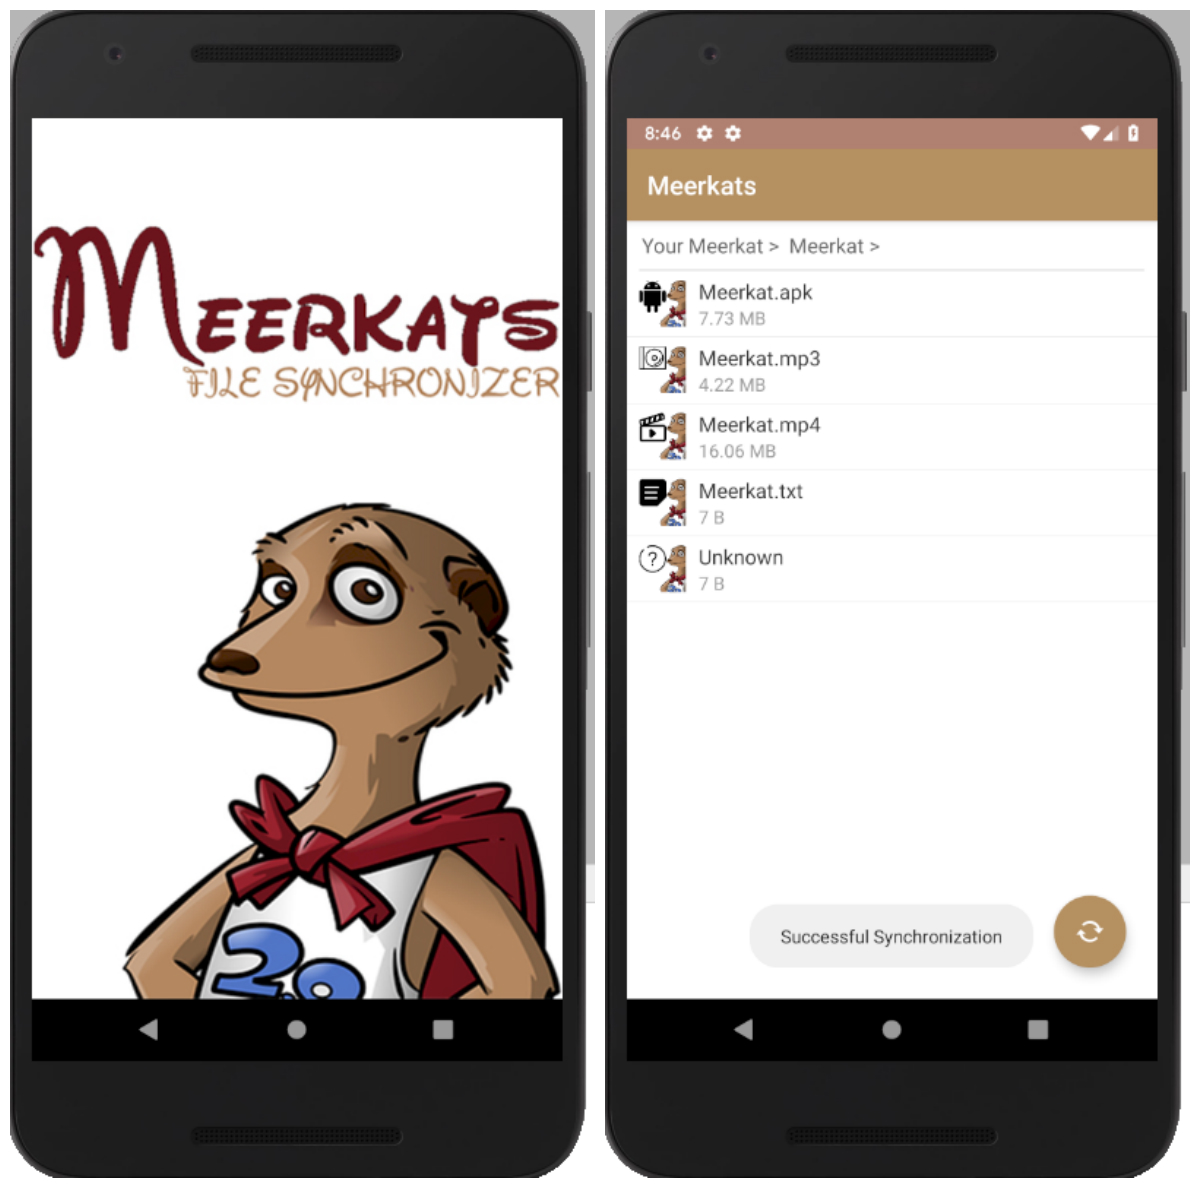
\includegraphics[width=0.95\textwidth]{collage1}
    \caption{Screenshots of the app in action}
    \label{fig:collage1}
\end{figure}

\subsection{Desktop Application Interface Design Principles}
As with mobile app interface design interface, our goal was to create a perfect user experience. We thoroughly thought of how to design desktop application interface that is simple to use, fun to interact with and intuitive. Some rules that we considered include the following:
\begin{itemize}
\item Combine what should be combined. Features that support the execution of a task have been gathered in one place. Consequently, tasks that are performed through multiple steps can be performed in streamlined flow.
\item Separate what should be separated. To support simplicity and avoid complex interface, key features are presented in very clear way while optional and secondary features are hidden. We also, separated tasks related to specific function (creation of a new file for example) from tasks supporting another function (uploading existing file).
\item Eliminate what can be eliminated. The interface design has been reviewed to examine the text and all elements to make sure that clear, simple and easy to understand words are used and no redundancy in the element.
\item Put the elements in the right place. We followed logical order when placing buttons and instructions. Progressive Disclosure Technique has been considered as applicable. It is about displaying additional information as needed instead of filing the home page with too many elements and information.
\item Use meaningful high-level combinations. It is often simpler and more scalable to select and manipulate groups of related elements than individual elements. Examples of high-level combinations include folders, themes, styles, and user groups. Such combinations often map to a user goal or intention that isn't apparent from the individual elements. For example, the intention behind the High Contrast Black color scheme is far more apparent than that of a black window background.
\item Select the right controls. Design elements have presented in efficient manner by selecting the right controls. We know that selecting the right controls are important to effectively interact with the application. For example, the saving file function has been presented in a simple dialog box that ask the users to enter the file name and type then have the options to save it or cancel the transaction.
\end{itemize}

\hfill \break
This flowchart, shown in Figure 4, shows the high level design of the software. The flow chart illustrates the main functions and the flow of the process. It is worth mentioning that the desktop and the mobile clients apply the same process flow.

\begin{figure}[H]
    \centering
    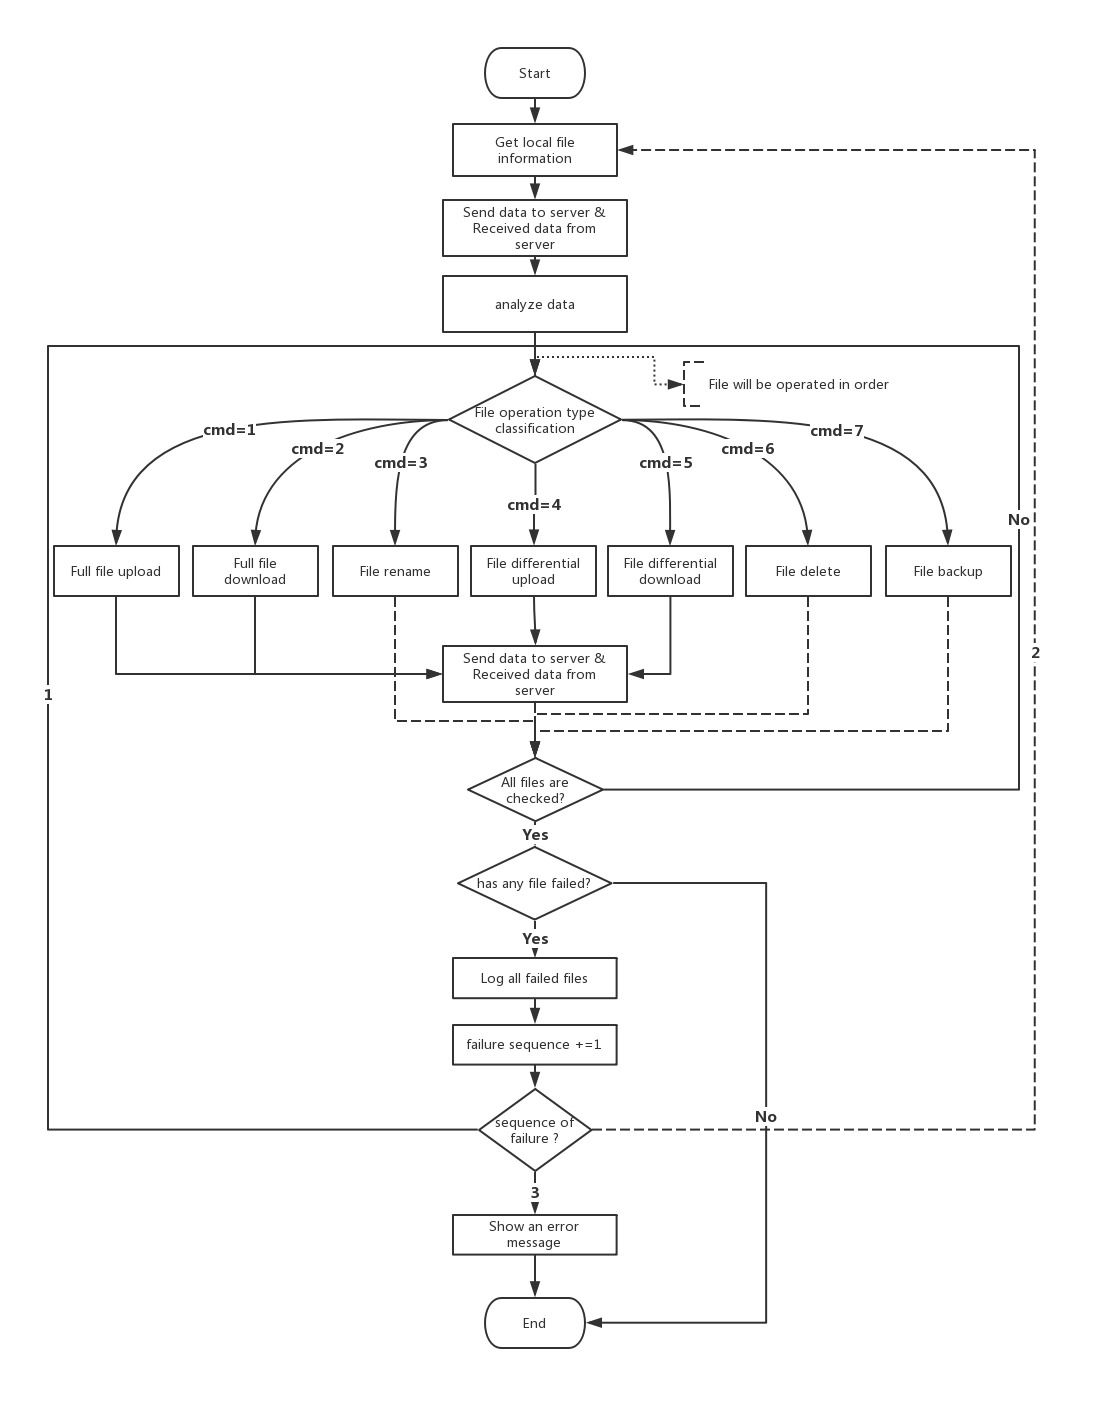
\includegraphics[width=0.95\textwidth]{flowchart}
    \caption{Client Solution Flowchart}
    \label{fig:flowchart1}
\end{figure}

\hfill \break

\subsection{Security Design}

The team worked hard to ensure not only delivering functional solution but also a secured product. For that, the team followed the security principles that were cited in Open Web Application Security Project (OWASP) Development Guide. They include:

\begin{enumerate}
\item \textbf{The principle of Defense in depth}
The principle of defense in depth is considered in the design. The team used different security controls to approach different risks such as data leakage, data unavailability, code injection, etc.
\begin{itemize}
\item \textbf{Process Title:} Establishing Secure Connection (Handshake)
\item \textbf{Risk:} Adversaries could intercept the connection between the client and the server and/or alter data or view sensitive data, in addition to repudiation risk.
\item \textbf{Security Control Title:} Rivest-Shamir-Adleman (RSA) Algorithm. RSA was used to provide secure connection and protection of data storage. The security of an algorithm depends on the length of the private key and since it is so far very difficult for attackers to compute large prime number, which is the result of multiplying two large primes we selected RSA.

\item \textbf{Process Title:} Key Exchange Stage through (Diffe-Hellman) Algorithm
\item \textbf{Risk:} Private keys can be accessed by unauthorized people, which could result in their ability to decrypt cipher text and get access to sensitive data in plaintext.
\item \textbf{Security Control:} Since we used RSA to encrypt the connection, it is very important to use secure method to exchange keys. We used Diffe-Hellman because it is a simple yet secured algorithm to facilitate key exchange.

\item \textbf{Process Title:} Data Stream Encryption through Advanced Encryption Standard (AES)
\item \textbf{Risk:} Data travel over the internet in plaintext format are vulnerable to many threats such as unauthorized access and potentially malicious modification by adversaries. To protect against those threats, we used AES to encrypt the communication between the server and the clients.
\item \textbf{Security Control:} Data Stream Cipher- Advanced Encryption Standards (AES). This cipher was used to encrypt data when they are streamed to the cloud.

\item \textbf{Process Title:} Securely Transmitting and Synchronizing Files
\item \textbf{Risk:} The integrity of files transferred over the Internet and stored in the web need to be protected from unauthorized modification and data manipulation.
\item \textbf{Security Control:} We are using a cryptographic hashing function ‘Message Digest (MD5) ‘ to validate data integrity when digitally transferred over the Internet. MD5 produces 128-bit hash value to check data integrity. We selected MD5 as it is simple to be implemented and we are considering using more secure non-cryptographic hash function such as MurMur in future since it has less structure considering the number of assembly instructions it generates as well as it provides a better collisions resistance than MD5.

\end{itemize}

\end{enumerate}

\section{Implementation}
The team has spent a great amount of time searching and deciding on the best approach to execute the project and the right methodology to develop the building blocks of the software and the integration among those components.

\subsection{Programming languages}
We discussed among the team what are the right languages to use to develop the server, mobile client and desktop app. We agreed on the following languages:
\begin{itemize}
\item\textbf{The Server:} The group decided to use Golang, also known as Go, for building the server. Golang is an open source programming language that makes it easy to build simple, reliable, and efficient software. Golang has great advantages, such as no pointer arithmetic, no manual memory management, a standard library that seems fairly well thought out and purposefully excludes things that are misused (ex. no ECB mode for AES).
\item\textbf{The Mobile Client:} Java was used to build the android mobile application. The reason for choosing Java is that it is a commonly used language and some of the team members are already familiar with it. Additionally, many development tools are available for Java. It is a popular object oriented programming language with most phones compatible with it.
\item\textbf{The Desktop Client:} C\# was selected to build the windows desktop application because it is targeted towards the windows operating system. Additionally, C\# has a built-in advanced code editor and debugger, which leads to easier debugging of errors. It also has an intensive framework, which makes developing the desktop client much more efficient.
\end{itemize}

\hfill \break
\textbf{Data Storage and Transmissions Method}
Serialization was used to enable data transmission between the devices. In computer science, in the context of data storage and transmission, serialization is the process of converting a data structure or object into a sequence of bits so that it can be stored in a file or memory buffer, or transmitted across a network connection link to be "resurrected" later in the same or another computer environment. There are two ways of transmitting data between server and browser and in which we can encode data. The two methods are JavaScript Object Notation (JSON) and Protocol Buffers, known as Protobuf. We decided to use JSON as it meets our technical needs and for simplicity and convenience. JSON uses Ajax to enable the exchange of data between the web application and the browser and server, without the need to reload the page and it encodes data in a human readable manner. However, in future version of the software, we might switch to Protobuf to overcome some limitations in JSON, such as the slowness of encoding and decoding for integers and floats. Comparing strings is a bit time consuming as well, as the need for sequential scan when parsing strings, arrays and objects which in all preceding cases are mitigated in Protobuf.

\hfill \break
\textbf{Communication Protocol}
The software is running over TCP protocol through port 4356. The team originally has thought of two protocols that are TCP and UDP as both of them are used to transfer data over the Internet. The decision was made to use TCP over UDP, and the main reason for this is that TCP is reliable and stateful protocol which is important feature to ensure complete and ordered transfer of file bits during download/upload stage.

UDP doesn’t guarantee delivery of data packets or even the sequence of which it has to be received plus it doesn’t establish end-to-end connection between communicating systems. For all these reasons we opted for TCP.
\newline
\hfill \break
\textbf{Compression Method(gzip)}
Gzip is both a file format and a software application that is used for file compression and decompression. HOW DO WE USE IT
\textbf{Rsync: An overview:} We have looked at Rsync as suggested by the project supervisor and found it to be sufficient to do the job. In a nutshell, Rsync is used to detect changes in files that are stored in two different locations and then sync the file in the remote sever to be identical to the file that is stored in local hard drive without the need to send the complete file over the internet to the server once again each time a user makes a change in the local version of it.
\newline
\hfill \break
\textbf{How it works:}
Below steps were copied from \underline{jenkov.com} as they well describe how rsync works.
\begin{enumerate}
\item The computer holding the newest version of the file is here called NEW, and the computer holding the oldest file is called OLD.
\item OLD divides the oldest version of the file into blocks of, say 1024 or 2048 bytes. The file is not divided on the disk. It's just something OLD does logically, internally in the memory.
\item For each block OLD calculates a checksum.
\item The list of block checksums are sent to NEW.
\item NEW searches the newest version of the file for blocks of data that has the same checksum as those found in the old version of the file. This is done by fist calculating the checsum for the very first block of data (1024 or 2048 bytes). If this checksum does not match any checksum in the old file, NEW moves 1 byte down the new file and calculates the checsum for this 1024 checksum. NEW thus calculates checksums for every possible 1024 (or 2048) byte block in the new file, to search for matches to blocks in the old file.
\item If NEW finds a 1024 byte block with the same checksum as one of the checksums received from OLD, then it considers that block to exist in the old version. It doesn't matter if the sequence of blocks is not the same as in the old version. NEW now skips to the end of this block and continues searching for checksum matches from there.
\item NEW will thus find X blocks of data matching checksums in the old file. This is the data that has not changed between the old and the new version of the file. In between these blocks will be data that was not part of a 1024 block that matched a checksum in the old file. This data is CHANGES, either new or modified data.
\item NEW sends back instructions to OLD on how to create a copy of the newest version of the file. NEW does this by sending a list of block references in the old file for the sections of the newest file that has not changed. For the parts that has changed NEW sends back the changed data in full.
\item OLD receives the list of block references and literal data (the changes), and from the old file and the literal data, constructs the new version of the file.
\end{enumerate}

\textbf{External Tools and libraries}
We are using the Git Feature Branch Workflow, meaning that all our development takes place in a dedicaded branch, and not in the master branch. This enables us to work on a specific feature without disturbing the main codebase. The biggest advangage is that we are keeping the master branch free from broken code. Our features include server, docs, android and desktop.

\subsection{Protocol}

We design a communication protocol over TCP. On both the server and client side, packets of a similar format are constructed and sent as TCP payload. By sending packets between the server and clients, we can communicate in an efficient and flexible way.

\begin{figure}[H]
    \centering
    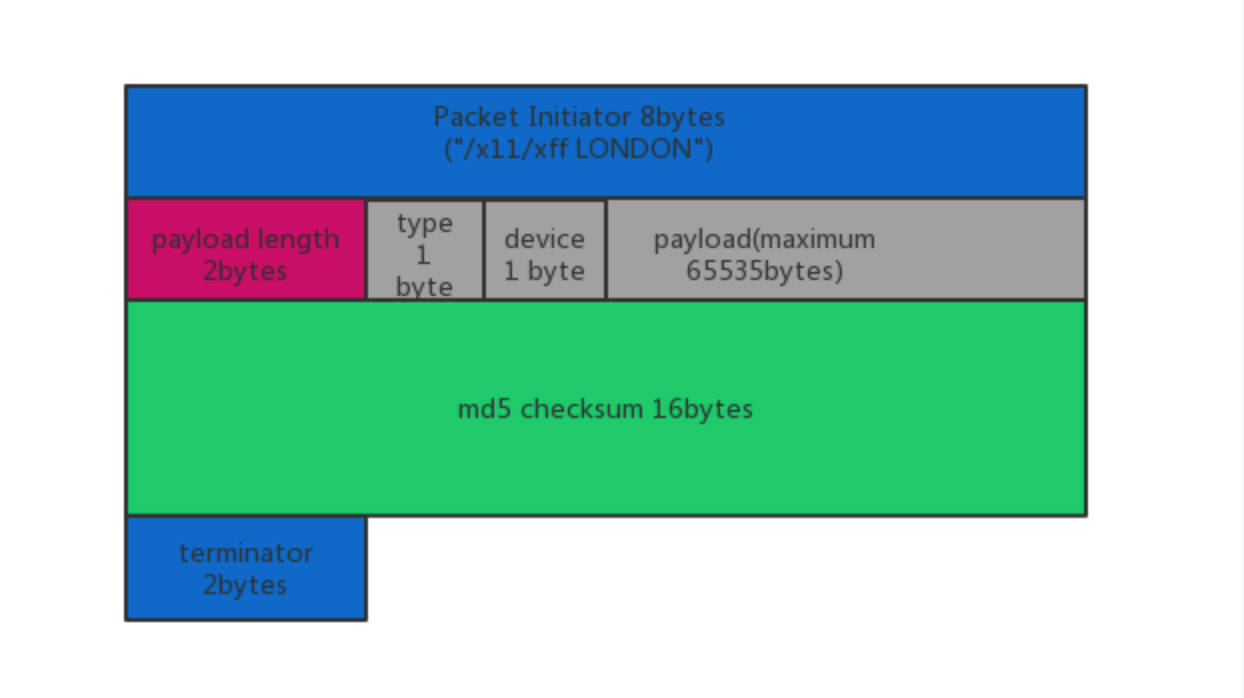
\includegraphics[width=0.95\textwidth]{packet}
    \caption{Packet structure}
    \label{fig:packet1}
\end{figure}

\begin{lstlisting}
blue area:initiator or terminator 8bytes
red area: payload length 2bytes
grey area:payload 0bytes-65535bytes
green area:checksum 16bytes
\end{lstlisting}

On server, we utilize a FSM to capture structured packets within the TCP stream and resolve them to extract data payload inside. The flowchart below demonstrates the working mechanism of the FSM that we implemented.
\newline
\hfill \break
For simplicit, we assume the initiator to be a two-byte value 0x110xff.

 \begin{figure}[H]
     \centering
     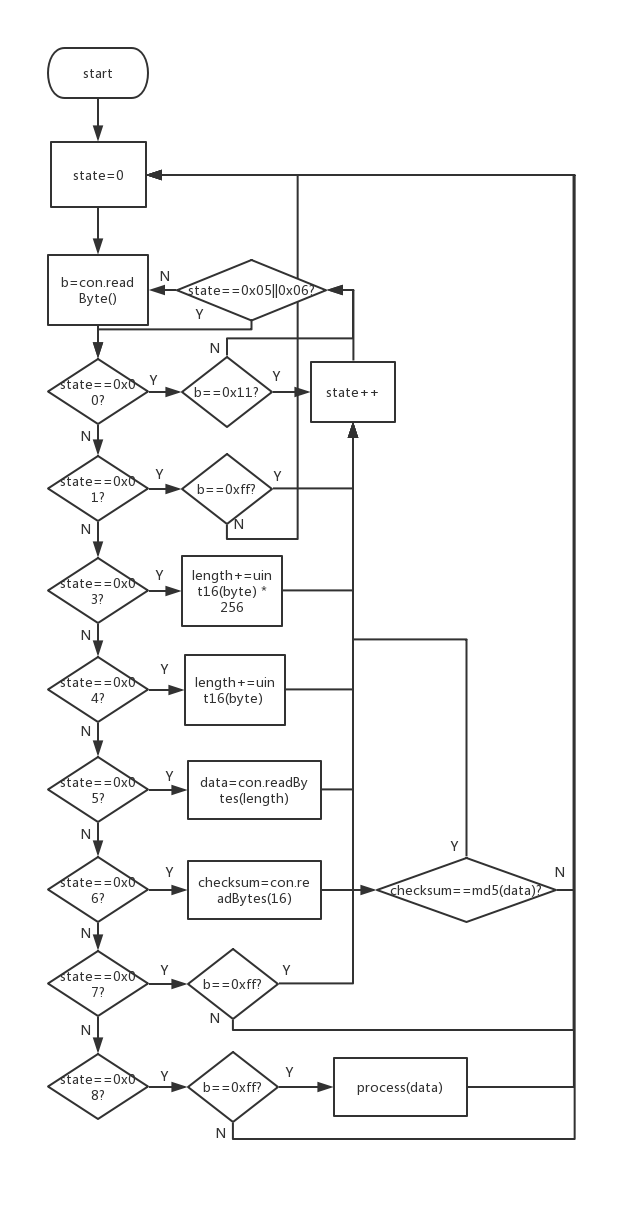
\includegraphics[width=0.95\textwidth]{protocolflowchart}
     \caption{FSM}
     \label{fig:protocolflowchart}
 \end{figure}

 With different type id, we can construct different types of packets.

 \begin{center}
 \begin{tabular}{ | m{2cm}  | m{2cm} | m{7cm} | }
 \hline
 \textbf{Type id} & \textbf{Name} & \textbf{Functionality} \\
 \hline
 0x02 & pull & Client scans the binded local dir and generates json formatted data that describes its structure. By sending the json to server, client acquires commands. Then it can manipulate local files according to these commands. \\
 \hline
 0x20 & download & Client sends a file index (index is sent over here with the above download command) to server, server responds with the file content (could be separated into multiple packets) \\
 \hline
 0x21 & upload & Client separates a file into pieces (if necessary) and sends them to server through a single packet or multiple packets. \\
 \hline
 0x22 & rdownload & Rsync download: Client separates a file into equal-sized blocks and calculate checksum for each block. Then it sends all these checksums to server. After receiving parts of the new file and some information indicating which blocks of the old file can be reused, client assembles a new file.
 \\
 \hline
 0x23 & rupload & Rysnc upload: Client receives sequence of checksums generated from the old versioned file as mentioned above. By comparing them to the latest versioned file, client can decide uploading which parts of the new file and will tell the server which blocks in the old versioned file can be reused. \\
 \hline
 \end{tabular}
 \end{center}

 From the perspective of a client, we will explain in detail how different types of packets are formed.
 \newline
 \hfill \break

\textbf{Pull packet:} After scanning locally, we know that there are two files in current directory, ”dir/doc1” and “pic1.jpg”, so the json below is formed.
 \begin{lstlisting}
 [{
 	"Name": "dir/doc1",
 	"Typ": 1,
 	"Digest": [62, 238, 247, 95, 134, 12,
             98, 97, 1, 23, 50, 153, 132,
             75, 115, 133]
 }, {
 	"Name": "pic1.jpg",
 	"Typ": 1,
 	"Digest": [141, 221, 57, 244, 109, 128,
            93, 240, 169, 147, 223, 23, 244,
            177, 183, 2]
 }]

 \end{lstlisting}

 Client encapsulates the json in a pull packet and sends it to server. Sever will then respond with a series of commands in the format of json (we will explain later how the server gives these commands).
 \newline
 \hfill \break
A possible reponse:

 \begin{lstlisting}
 [{
 	"Name": "pic1.jpg",
 	"Digest": [141, 221, 57, 244, 109, 128, 93, 240,
  169, 147, 223, 23, 244, 177, 183, 2],
 	"Cmd": 1,
 	"Ext": ""
 }, {
 	"Name": "dir/doc1",
 	"Digest": [62, 238, 247, 95, 134, 12, 98, 97,
   1, 23, 50, 153, 132, 75, 115, 133],
 	"Cmd": 1,
 	"Ext": ""
 }]
 \end{lstlisting}

Because the client has received two “command 1”, it should upload the two files immediately.
\newline
\hfill \break

All possible values in Cmd field:
 \begin{center}
 \begin{tabular}{ | m{1.4cm}| m{10cm} | }
 \hline
 \textbf{Cmd} & \textbf{Action}  \\
 \hline
  1 & Client should upload the related file.  \\
 \hline
 2 & Client should download the related file.  \\
 \hline
 3 & Client should rename the related file with the new name in “Ext” field. \\
 \hline
 4 & Client should upload the related file by using rsync algorithm. \\
 \hline
 5 & Client should download the related file by using rsync algorithm. \\
 \hline
 6 & Client should delete the related file. \\
 \hline
 7 & Client should backup the related file (move to a specific directory). \\
 \hline
 \end{tabular}
 \end{center}

 \textbf{Download packet and Upload packet:} No matter if it is a download packet or an upload packet, we transfer the files in a similar way. We will introduce the way we separate files and encapsulate packets in the following part.
 \newline
 \hfill \break
Because we use a two-byte value to record the payload length, its theoretical maximum length is 65535 (Except for the field of device id and the field of packet type). We also need to attach file information on each packet, so we pre-allocate another 300 bytes at the beginning of each packet. Therefore, we can transfer 65233 bytes at most in one packet. In other words, if the size of file is more than 65233 bytes, we have to send it in multiple packets.
\newline
\hfill \break
An example of file information json:

\begin{lstlisting}
{
	    "Name": "pic1.jpg",
	    "Num": 2,
	    "Index": 0
 }
\end{lstlisting}

This json means we send “pic1.jpg” in two separate packets (Num), and it is the first one (Index). Apparently, this json is no more than 300 bytes so we will have to pad the rest part with 0x00.
\newline
\hfill \break
The payload structure of a download or upload packet:

 \begin{figure}[H]
     \centering
     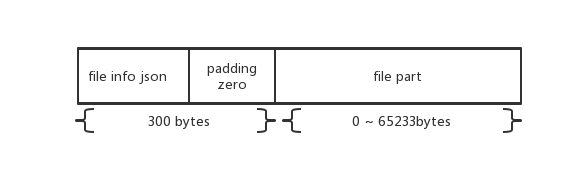
\includegraphics[width=1.1\textwidth]{payload-structure}
     \caption{The payload structure of a download or upload packet}
     \label{fig:payload-structure}
 \end{figure}

 \textbf{RSync packet:} When the client is told that its local file has been modified, it will use the rsync algorithm to download the file, rather than downloading a full file. On the contrary, if the user modified a file locally, client will use rsync to partly upload new file to server. By using rsync, we can reduce network data that is transmitted.
 \newline
 \hfill \break
Comparing stage:
Based on the previous version of the file, we can calculate hashes of every 1024-bit block. If the last block is less than 1024 bits in length, we should just ignore it. After sending these values of hash to the opposite side, we can compare to determine in the newest version of file how many blocks which contained unmodified value can be matched. Once these blocks are identified, we only need to transmit these unrepeated bits to the old-versioned side.
\newline
\hfill \break
Reassembling stage:
We convert the old version to the new version according to the below json list. When the “Typ” field evaluates to 1, it means this part of file is a modified part in the new version and we have to transmit it. The part  starts from offset “Idx” and has a length of “Len” bits.However, when the “Typ” field evaluates to 2, it means this part is a previous part that can be reused. It is the first block in the old version of file because the “Idx” equals to 0 in the example. In other words, Idx has two different meanings in the two different types of cases.

\begin{lstlisting}
[
   {
      "Typ":1,
      "Idx":0,
      "Len":1
   },
   {
      "Typ":2,
      "Idx":0,
      "Len":1024
   },
   {
       "Typ":1,
       "Idx":1025,
       "Len":10
   }
]

\end{lstlisting}

 \begin{figure}[H]
     \centering
     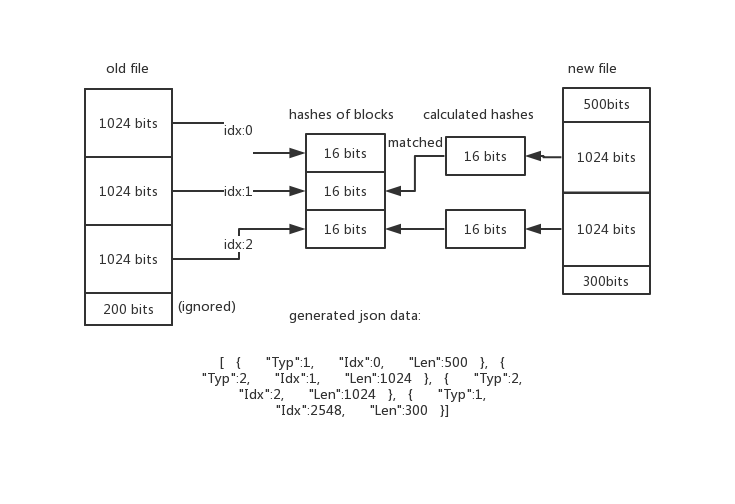
\includegraphics[width=1.1\textwidth]{reassembling-stage}
     \caption{}
     \label{fig:reassembling-stage}
 \end{figure}


\section{Team work}
Our team strongly believes on the principle "The whole is greater than the sum of its parts". The team consists of six students, and throughout the project lifecycle, we tried to tap into each individuals strength, and challenge each other to gain new knowledge. We aimed to make this expedience as enjoyable, yet beneficial, as possible.

\subsection{Effective Communication}
When we first got together, we discussed the importance of setting communication ground rules. We all come from different backgrounds and are used to different cultures. For that purpose, we developed "Communication Ground Rules", of which the team agreed to fully abide by those rules. The rules aimed to reduce the possibility of misunderstanding, conflicts and to ensure commitment and respect among the team.

Here are the group’s communication ground rules:
\begin{enumerate}
  \item Mutually commit to our team’s objectives as stated in the project report or negotiate until we can make this mutual commitment.
  \item All team members are expected to attend team meetings unless they are out of town or sick. If a team member is unavailable, he or she should notify the rest of the team and should share their update through email or Skype.
  \item Team meetings will start and end on time.
  \item Action items will be distributed within 24 hours after the meeting.
  \item Understand each other’s styles.
  \item Tackle issues, not people.
  \item Permit one speaker at a time (avoid side conversations).
  \item Bring issues to the table during the team update meeting.
  \item Explain the reasoning leading to your conclusions.
  \item Invite inquiry into your views.
  \item Inquire into the reasoning of others.
\end{enumerate}


Furthermore, the team depended on Google Docs to share links and important updates, and GIT to store project documentations. We also utilized technology such as Slack to facilitate instant conversation and to share information about the project, which has significantly saved everyone’s time.

\subsection{Conflict Management}
The team members were inspired to provide a friendly project environment that enabled everyone to put in their best efforts. We aimed to build a resilient team that responded to challenges, unforeseen events and different circumstances in a timely manner.

One way to avoid conflict was to use consensus for important decisions and issues. For less important issues, we relied on the subject matter expert with input from others. This approach worked well throughout the entire project.


\hfill \break %dont remove this line for some reason
The team also considered this group project as an opportunity to build the following types of skills:


\begin{itemize}
\item \textbf{Communication Skills:} Good communication skills are the most basic skills that one can possess as an employee or student. We aim to improve the team members ability to communicate effectively with each others and to convey information in a simple and unambiguous way.
\item \textbf{Practice Diversity:} The team consists of 6 members who come from different countries, speak different languages and have different backgrounds. We aim to learn how to recognize individual differences and understand how cultural differences can impact how people work, and interact.
\item \textbf{Project Management Skills:} Take this project as an opportunity to build project management skills that are essential to successfully complete a project that includes but not limited to planning, leadership, communication, and risk management.
\item \textbf{Teamwork Skills:} Teamwork is important for the success of this project. We aim to build teamwork skills, which are essentials at work after graduation. Each member will learn how to be a good team player by demonstrating skills such as negotiation, communication, problem solving and prioritization.
\end{itemize}

\section{Evaluation}
As expected, we had to do some changes here and there during the development stage for different reasons such as better performance, better user experience, more secure approach…etc.

In the desktop and mobile apps, the user input was through one variable only such as file name or the file type, then we decided to improve this logic to allow users to provide more variables at the same time to simplify the data input process.

\subsection{Mobile App Assessment}

\textbf{Design}
\begin{itemize}
\item We believed that the mobile interface is simple and intuitive, however, we did an initial assessment for the design and we had to change it. In the beginning we used a nice theme that represents the team goal of collaboration. However, it was realized that following this design is not practical when developing the pages that are intended to execute the entire functions. The feel and look of the mobile app has been changed to be in the context of file manger system.
\item Another point to highlight about the design it is compatible with any new version of android system, which extends its value and usability. Additionally, we carefully choose icons that can be adapted to any Dots Per Inch (DPI) this is very important to ensure that photos are displayed with a perfect resolution in any android devices regardless of what OS version or the size of the screen.
\item We used Splash Page to provide excellent first impression and to allow sometime for the application to do data caching in the background so users are entertained with the splash page and not feeling bored waiting for the application to start.
\item We provided default root directory (Your Meerkat) for security and convenience reasons. By implementing this control, users can’t navigate to other directory to store their files, which means they are always required to use the default directory, which we made sure to secure it. It also provides convenience, as users don’t have to navigate their device to allocate the file directory.
\end{itemize}

A general observation we would like to add is that we did partial testing but we couldn’t do complete cycle of testing for the software as we were running out of time. However, we tested some core functions and services such as resolving network packets and file synchronization.

\textbf{Functionality:}
Mobile app was developed using Java and that led to efficient implementation of the application this is rooted to the abundance of information and communities that share their knowledge about Java. For example, there was a difficulty in setting the IO function to enable reading exact length of data size from the server via TCP socket and with the assistance of Java online community the problem was resolved.

Some file management processes such as file rename and file deletion are executed by other applications and not through the mobile version of Meerkats that are due to challenging time needed to develop those features plus our skills in developing Android application require additional training to develop such advanced feature.


\textbf{Data Security}

The software is secured in general, the confidentiality, integrity and availability have been considered during the development work. However, the security level can be evolved in future to include more controls such as performing virus scanning when uploading/downloading files. Files’ content also, can be encrypted while stored in the server to avoid data leakage risk.

\section{Peer assessment}
The team agreed to distribute the 100 score by each one equally as showing in the following table. The rationale behind this decision is due to great efforts been put by everyone and as a reward for the continues commitment and hard work.


\begin{center}
\begin{tabular}{ | m{3cm}| m{1.3cm} | }
\hline
\textbf{Name} & \textbf{Points}  \\
\hline
Boyang Zhang & 16.66  \\
\hline
Xi He & 16.66  \\
\hline
YiFeng Zheng & 16.66 \\
\hline
Yenan Huang & 16.66 \\
\hline
Frida Solheim & 16.66 \\
\hline
Samah Alghamdi & 16.66 \\
\hline
\end{tabular}
\end{center}


\section{Challenges}
\begin{itemize}
\item \textbf{Communication:} Since we came from different background and since we speak different languages (Arabic, Chinese and Norwegian), having the ability to speak English clearly and be able to deliver information and updates in clear manner is vital to the success of the group. Our chines colleagues had a problem with demonstrating the ability to which resulted sometimes in miscommunication. \textbf{Solution:} We agreed to use very simple English words and terms when we discuss project update or argue ideas and that every one should ensure that his/her message has been delivered to every one correctly by using assurance questions such as am I clear? Did you understand my point? do you want me to repeat what I just said?...etc.

\item \textbf{Attendance Punctuality} In addition to our daily chats through slack, we decided to meet in person once every week to discuss progress, issues and better connect with each other’s. However, we had to cancel some meetings due to either tardiness of last minute notice of absence by some of the team members.
\textbf{Solution:} We created a process to address this issue. We agreed to deduct points from the peer-to-peer assessment scores if a member was late for more than 5 minutes of the meeting start time or didn’t inform the group about his/her absence 24 hours prior the meeting date. This process ensured timely attendance and commitment of all team members.
\item \textbf{Project timeframe:} Although the project’s supervisor provided clear requirements, the implementation was a bit challenging due to different reason one is the project duration. In addition to work on the project, the team members had to attend lectures and work on other course works related to other modules as well as started to work on the dissertation to sit the scope of work and agree on the course of actions with the dissertation supervisor, which put the team members under pressure.
\textbf{Solution:} We divided the work and sat priorities before starting any new tasks. We jumped to assist each other’s when anyone get stuck in task in hands. We tried to deliver the main requirements and decided to include features that we didn’t find the time to execute as future work.
\item \textbf{Handling Technical Issues:} Description: Developing mobile application was a new experience and for that we tried our best to learn how to develop android application but we encountered many technical issues for which we used online resources to solve them, however, some problems are too complicated and we still figuring out how to address them. For example, context is an important concept and feature in Android development. We have to learn it from scratch and it was really difficult. However, we managed to develop the basic requirements such as synchronization feature but we believe that there is an area for improvement in future.
Another problem is about how to bind the code with design. All these are new to us and they took a lot of time yet we still didn’t make them perfect.
\textbf{Solution:} We used all possible online resources and communities such as Stackoverflow to ask questions and/or search for answers for problems that were encountered by others. We also used Github to look into source codes to apply similar concept in our code. We also used online videos to learn how to bind code with design and we managed to address this problem too.

\end{itemize}

\section{Future Work}
\begin{itemize}

\item \textbf{Design iPhone client}
\textbf{Description:} In addition for the software to be compatible with Windows and Android, we are planning to further enhance its usability by developing MAC client.
\textbf{Added Value:} More users especially those who have iphones and mac desktops are expected to use the software and benefit from its services.

\item \textbf{Development of Privacy Policy Statement}
\textbf{Description:} Devise private statement explaining how are we storing the user’s files, for how long, what happens when the retention date is approached and what controls we apply to protect them and then require user’s consent for allowing us to store their data on our cloud and that they are in agreement with how are protecting their data.
\textbf{Added Value:} with the introduction with GDPR, it is crucial to let users’ know how their data is being dealt with by us and obtain their consent accordingly to avoid any legal implications that may occur in future in case of any data breach incidents that are a result of users’ mistakes not due to a vulnerability in our system.


\item \textbf{Introduction of Authentication Feature:} Currently, the application is automatically accessible by the two clients (mobile and desktop), which is a basic requirement by the project. Our plan is to make the software available to public users, it is imperative to introduce user’s authentication feature to protect the confidentiality of each users. The design will also be improved by adding users’ sign up page.
\textbf{Added value:} Better information security by authenticating users.

\item \textbf{Allocation of Individual Disk Space:} We aim to make the application available to public and for that we need to allocate default storage space for each users which can be expanded in future by purchasing more space. Space allocation will be dynamic to enhance server performance by utilizing the memory space in sufficient manner.
\textbf{Added Value:} Better users experience by giving users the opportunities to increase their storage space on paid fashion as well as optimized server performance.


\item \textbf{Introduce file versioning feature}
\textbf{Description:} File versioning feature enables archiving the old version of a file when users attempt to delete it or replace it with a newer version and still want to keep the old versions of the original file. This feature will be configured per file and on per-device fashion and it is usually defaulted to no file versioning are used.
We will decide on the file versioning strategies and will be using one of the available options such as automatically delete files if they are older than the maximum age or exceed the number of files allowed in an interval (one hour, one day, 30 days). Another strategy is to delegate file versioning method to an external program after specifying the versioning strategies.
\textbf{Added Value:} Since dealing with electronic documents involved rapid changes, there is a need to keep old versions to restore deleted files or undo certain changes. It will also, increase collaboration among team members who might be working on the same project as each person will have the chance to work on the same file at the same time and all versions will be kept in one repository.


\item \textbf{Anticipate and Answer Users’ Queries:}
\textbf{Description:} When users tap a button, they want to know whether the process has started and how long will it take. As technology abstracts these actions, the users are usually kept in the dark while the process is going on. Use Toast in Android and notifications in iOS so users will be notified when a process has completed. The Gmail app is a good example of such a design, as it displays messages like “saved in draft, message sent, etc.” to inform the users about the completion of the task.
\textbf{Added Value:} better user experience as users can anticipate how long it will take to complete their request and better manage their times.

\item \textbf{Application Feel and Look:} Since it is important to deliver simple yet enjoyable user experience, we will continue to do general improvement from interface perspective by make it more interactive and attractive for example, we are thinking to use Meerkats icon as a dynamic command button that responds to users’ clicks so users don’t feel bored while waiting for their transactions to be completed.
\textbf{Added Value:} Increase user satisfaction and retention.

\end{itemize}

\section{Things I am adding later/working on}
Finite-State Matchine(FSM)
What is a FSM?
Our server implements a FSM model to process incoming TCP stream of bytes.
You can find out what my implementation is in the part of “Pseudocode For Depacking”. (http://t.cn/EIi6Kxs)

\nocite{*}

\bibliography{final-report}
\bibliographystyle{plainurl}


\end{document}
